\begin{frame}{potentially unwanted programs (PUP)}
    \begin{itemize}
    \item most commonly: programs bundled with other programs
    \item sometimes disclosed but in (deceptive?) fine print
    \item sometimes considered malware, sometimes not
    \end{itemize}
\end{frame}

\begin{frame}{bad behavior by `normal' programs}
    \begin{itemize}
    \item some mostly-legitimate programs also do malware-like things
    \vspace{.5cm}
    \item location info collected by cell phone apps?
    \item advertisments injected by useful browser extensions?
    \end{itemize}
\end{frame}


{ % all template changes are local to this group.
    \setbeamertemplate{navigation symbols}{}
    \begin{frame}[plain]
        \begin{tikzpicture}[remember picture,overlay]
            \node[at=(current page.center)] {
                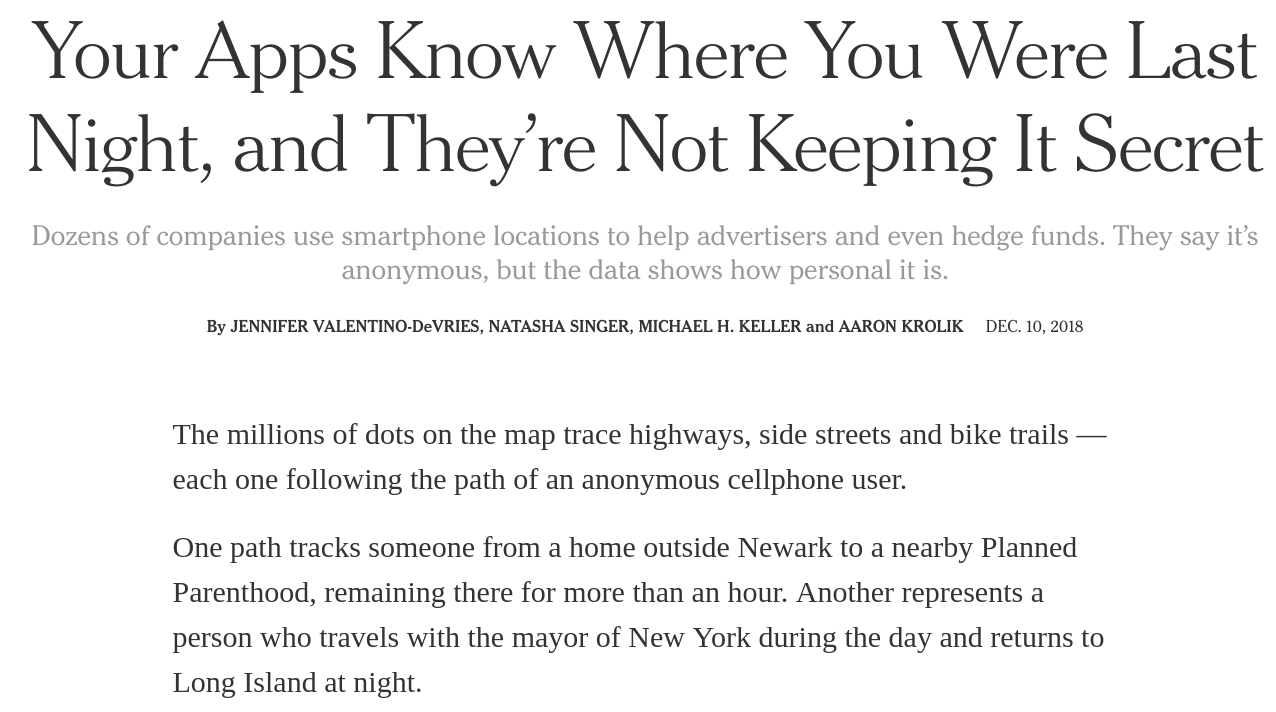
\includegraphics[width=\paperwidth]{../intro/app-location-data-art}
            };
        \end{tikzpicture}
    \end{frame}
}
